In this chapter we will evaluate the architectures described in chapter \ref{chapter:architectures} with the method described in chapter \ref{chapter:design_of_experiments}. Some of them will additionally be evaluated with the implementation from chapter \ref{chapter:implementation}.






\section{Assumptions}
\subsection{Bandwidth}
When evaluating we are making some assumptions about bandwidth. Table \ref{tab:Bandwidth_latency} shows latency and bandwidth for different technologies. The WiFi bandwidths are based on data from CenturyLink\cite{noauthor_24_nodate}. The 4G and 5G bandwidths are real-world examples from 4g.co.uk\cite{noauthor_how_nodate}. The 4G latency are from ping tests, while the 5G latency are from Verizon\cite{noauthor_what_2020}.

\begin{table}[h!]
    \centering
    \begin{tabular}[c]{|c|c|c|}
        \hline
        Technology & Latency (ms) & Bandwidth (Mbps) \\
            &   &  Download/Upload \\
        \hline
        \hline
        Wifi (2.4GHz) & <=1 & 150/150  \\
        \hline
        Wifi (5GHz) & <=1 & 450/450  \\
        \hline
        4G & 30-65 & 42/25  \\
        \hline
        5G & 30 & 200/100  \\
        \hline
        Wired LAN & <=1 & 1000+  \\
        \hline
        WAN & 10-300+ & 1000+  \\
        \hline
        
        
    \end{tabular}
    \caption{Latency and bandwidth for different technologies.}
    \label{tab:Bandwidth_latency}
\end{table}
When doing calculations in this chapter, we will be using numbers from table \ref{tab:Bandwidth_latency}.




\subsection{Hardware}
According to cpubenchmark\cite{noauthor_passmark_nodate}, flagship phones is about half as fast as a standard desktop CPU. We assume that we are dealing with below average CPU's cellphones, as most people do not have the flagship phone. We will test different strengths of the MEC Server. We assume that the data centre will have plenty of resources. In total, we want to do 10000 iterations spread over all the nodes.




\subsection{Local execution}
%lacking geographic location?
\begin{table}[h!]
    \centering
    \begin{tabular}[c]{|c|c|c|c|}
        \hline
        Node type & Limitation & Iterations & Time used (s) \\
        \hline
        \hline
        Local & 30 & 10000 & 333.6 \\
        \hline
    \end{tabular}
    \caption{Only local execution.}
    \label{tab:MEC_local_execution}
\end{table}
Table \ref{tab:MEC_local_execution} shows the time used for local execution only.


\subsection{Common results}
The tables shown in the following two sub subsections are common for both MEC and Cloudlets. This is because we test the same hardware, so when latency is not a factor, we will have the same results. They are all results of tests with little to no latency.

\subsubsection{Full offloading}
%spread out over more nodes
\begin{table}[h!]
    \centering
    \begin{tabular}[c]{|c|c|c|c|}
        \hline
        Node type & Limitation & Iterations & Time used (s)\\
        \hline
        \hline
        Local & 30 & 0 & 0 \\
        \hline
        Near & 100 & 2500 & 23.3 \\
        \hline
        Far & 300 & 7500 & 30.5 \\
        \hline
    \end{tabular}
    \caption{Full offloading.}
    \label{tab:MEC_full_offloading}
\end{table}

\begin{table}[h!]
    \centering
    \begin{tabular}[c]{|c|c|c|c|}
        \hline
        Node type & Limitation & Iterations & Time used (s)\\
        \hline
        \hline
        Local & 30 & 0 & 0 \\
        \hline
        Near & 100 & 2800 & 27.3 \\
        \hline
        Far & 300 & 7200 & 29.8 \\
        \hline
    \end{tabular}
    \caption{Full offloading with more balance.}
    \label{tab:MEC_full_offloading_balanced}
\end{table}

Table \ref{tab:MEC_full_offloading} and \ref{tab:MEC_full_offloading_balanced} shows time used when offloading work to nodes that have little to no latency from Local (less than 1 ms). This essentially shows how much time is used on calculation if we have no communication between nodes. 

\subsection{Partial offloading}
The tables shown in this subsection are common for both MEC and Cloudlets. This is because we test the same hardware, so when latency is not a factor, we will have the same results.
\begin{table}[h!]
    \centering
    \begin{tabular}[c]{|c|c|c|c|}
        \hline
        Node type & Limitation & Iterations & Time used (s)\\
        \hline
        \hline
        Local & 30 & 1000 & 33.0 \\
        \hline
        Near & 100 & 2000 & 19.5 \\
        \hline
        Far & 300 & 7000 & 30.6 \\
        \hline
    \end{tabular}
    \caption{Partial offloading.}
    \label{tab:MEC_partial_offloading}
\end{table}


\begin{table}[h!]
    \centering
    \begin{tabular}[c]{|c|c|c|c|}
        \hline
        Node type & Limitation & Iterations & Time used (s)\\
        \hline
        \hline
        Local & 30 & 850 & 28.1 \\
        \hline
        Near & 100 & 2700 & 26.5 \\
        \hline
        Far & 300 & 6450 & 29.1 \\
        \hline
    \end{tabular}
    \caption{Partial offloading with more balance.}
    \label{tab:MEC_partial_offloading_balanced}
\end{table}
Table \ref{tab:MEC_partial_offloading} and \ref{tab:MEC_partial_offloading_balanced} shows the result of offloading with less than 1 ms latency and little overhead.






\section{Multi-Access Edge Computing} \label{section:MEC_evaluation}

\subsection{Full offloading}
\begin{table}[h!]
    \centering
    \begin{tabular}[c]{|c|c|c|c|c|}
        \hline
        Node type & Limitation & Iterations & RTT to Local (ms)& Time used (s)\\
        \hline
        \hline
        Local & 30 & 0 & 0 & 0 \\
        \hline
        Near & 100 & 2800 & 30 & 92.8 \\
        \hline
        Far & 300 & 7200 & 170 & 1304.8 \\
        \hline
    \end{tabular}
    \caption{Full offloading with communication between Local and Near/Far.}
    \label{tab:MEC_full_offloading_latency}
\end{table}

Table \ref{tab:MEC_full_offloading_latency} shows how latency affects the work. Here, it will have to get data from Local after every iterations. There is a lot of communication between the nodes.

\begin{table}[h!]
    \centering
    \begin{tabular}[c]{|c|c|c|c|c|}
        \hline
        Node type & Limitation & Iterations & RTT to Local (ms)& Time used (s)\\
        \hline
        \hline
        Local & 30 & 0 & 0 & 0 \\
        \hline
        Near & 100 & 8500 & 30 & 279.3 \\
        \hline
        Far & 300 & 1500 & 170 & 267.9 \\
        \hline
    \end{tabular}
    \caption{Full offloading with communication and more balance in the nodes.}
    \label{tab:MEC_full_offloading_latency_balance}
\end{table}

Table \ref{tab:MEC_full_offloading_latency_balance} shows a more balanced workload distribution. The Near node is doing significantly more work. Here we also have to get data from Local after each iteration.














\subsection{Partial offloading}




\begin{table}[h!]
    \centering
    \begin{tabular}[c]{|c|c|c|c|c|}
        \hline
        Node type & Limitation & Iterations & RTT to Local (ms)& Time used (s)\\
        \hline
        \hline
        Local & 30 & 850 & 0 & 28.1 \\
        \hline
        Near & 100 & 2700 & 30 & 86.0 \\
        \hline
        Far & 300 & 6450 & 170 & 1131.2 \\
        \hline
    \end{tabular}
    \caption{Partial offloading with communication between Local and Near/Far.}
    \label{tab:MEC_partial_offloading_latency}
\end{table}

Table \ref{tab:MEC_partial_offloading_latency} shows how latency affects offloading. We have the same configuration as shown in table \ref{tab:MEC_partial_offloading_balanced}, but now the nodes are spread out and have latency affecting the offloading. The nodes have to get data from Local after each iteration.

\begin{table}[h!]
    \centering
    \begin{tabular}[c]{|c|c|c|c|c|}
        \hline
        Node type & Limitation & Iterations & RTT to Local (ms)& Time used (s)\\
        \hline
        \hline
        Local & 30 & 4550 & 0 & 151.3  \\
        \hline
        Near & 100 & 4525 & 30 & 149.8 \\
        \hline
        Far & 300 & 925 & 170 & 163.0 \\
        \hline
    \end{tabular}
    \caption{Partial offloading with communication and more balance in the nodes.}
    \label{tab:MEC_partial_offloading_latency_balance}
\end{table}


Table \ref{tab:MEC_full_offloading_latency_balance} shows a more balanced version. We can see that more of the work happens locally and on the node with less latency.

\subsection{Decreasing interaction}

\begin{figure}[t]
    \centering
    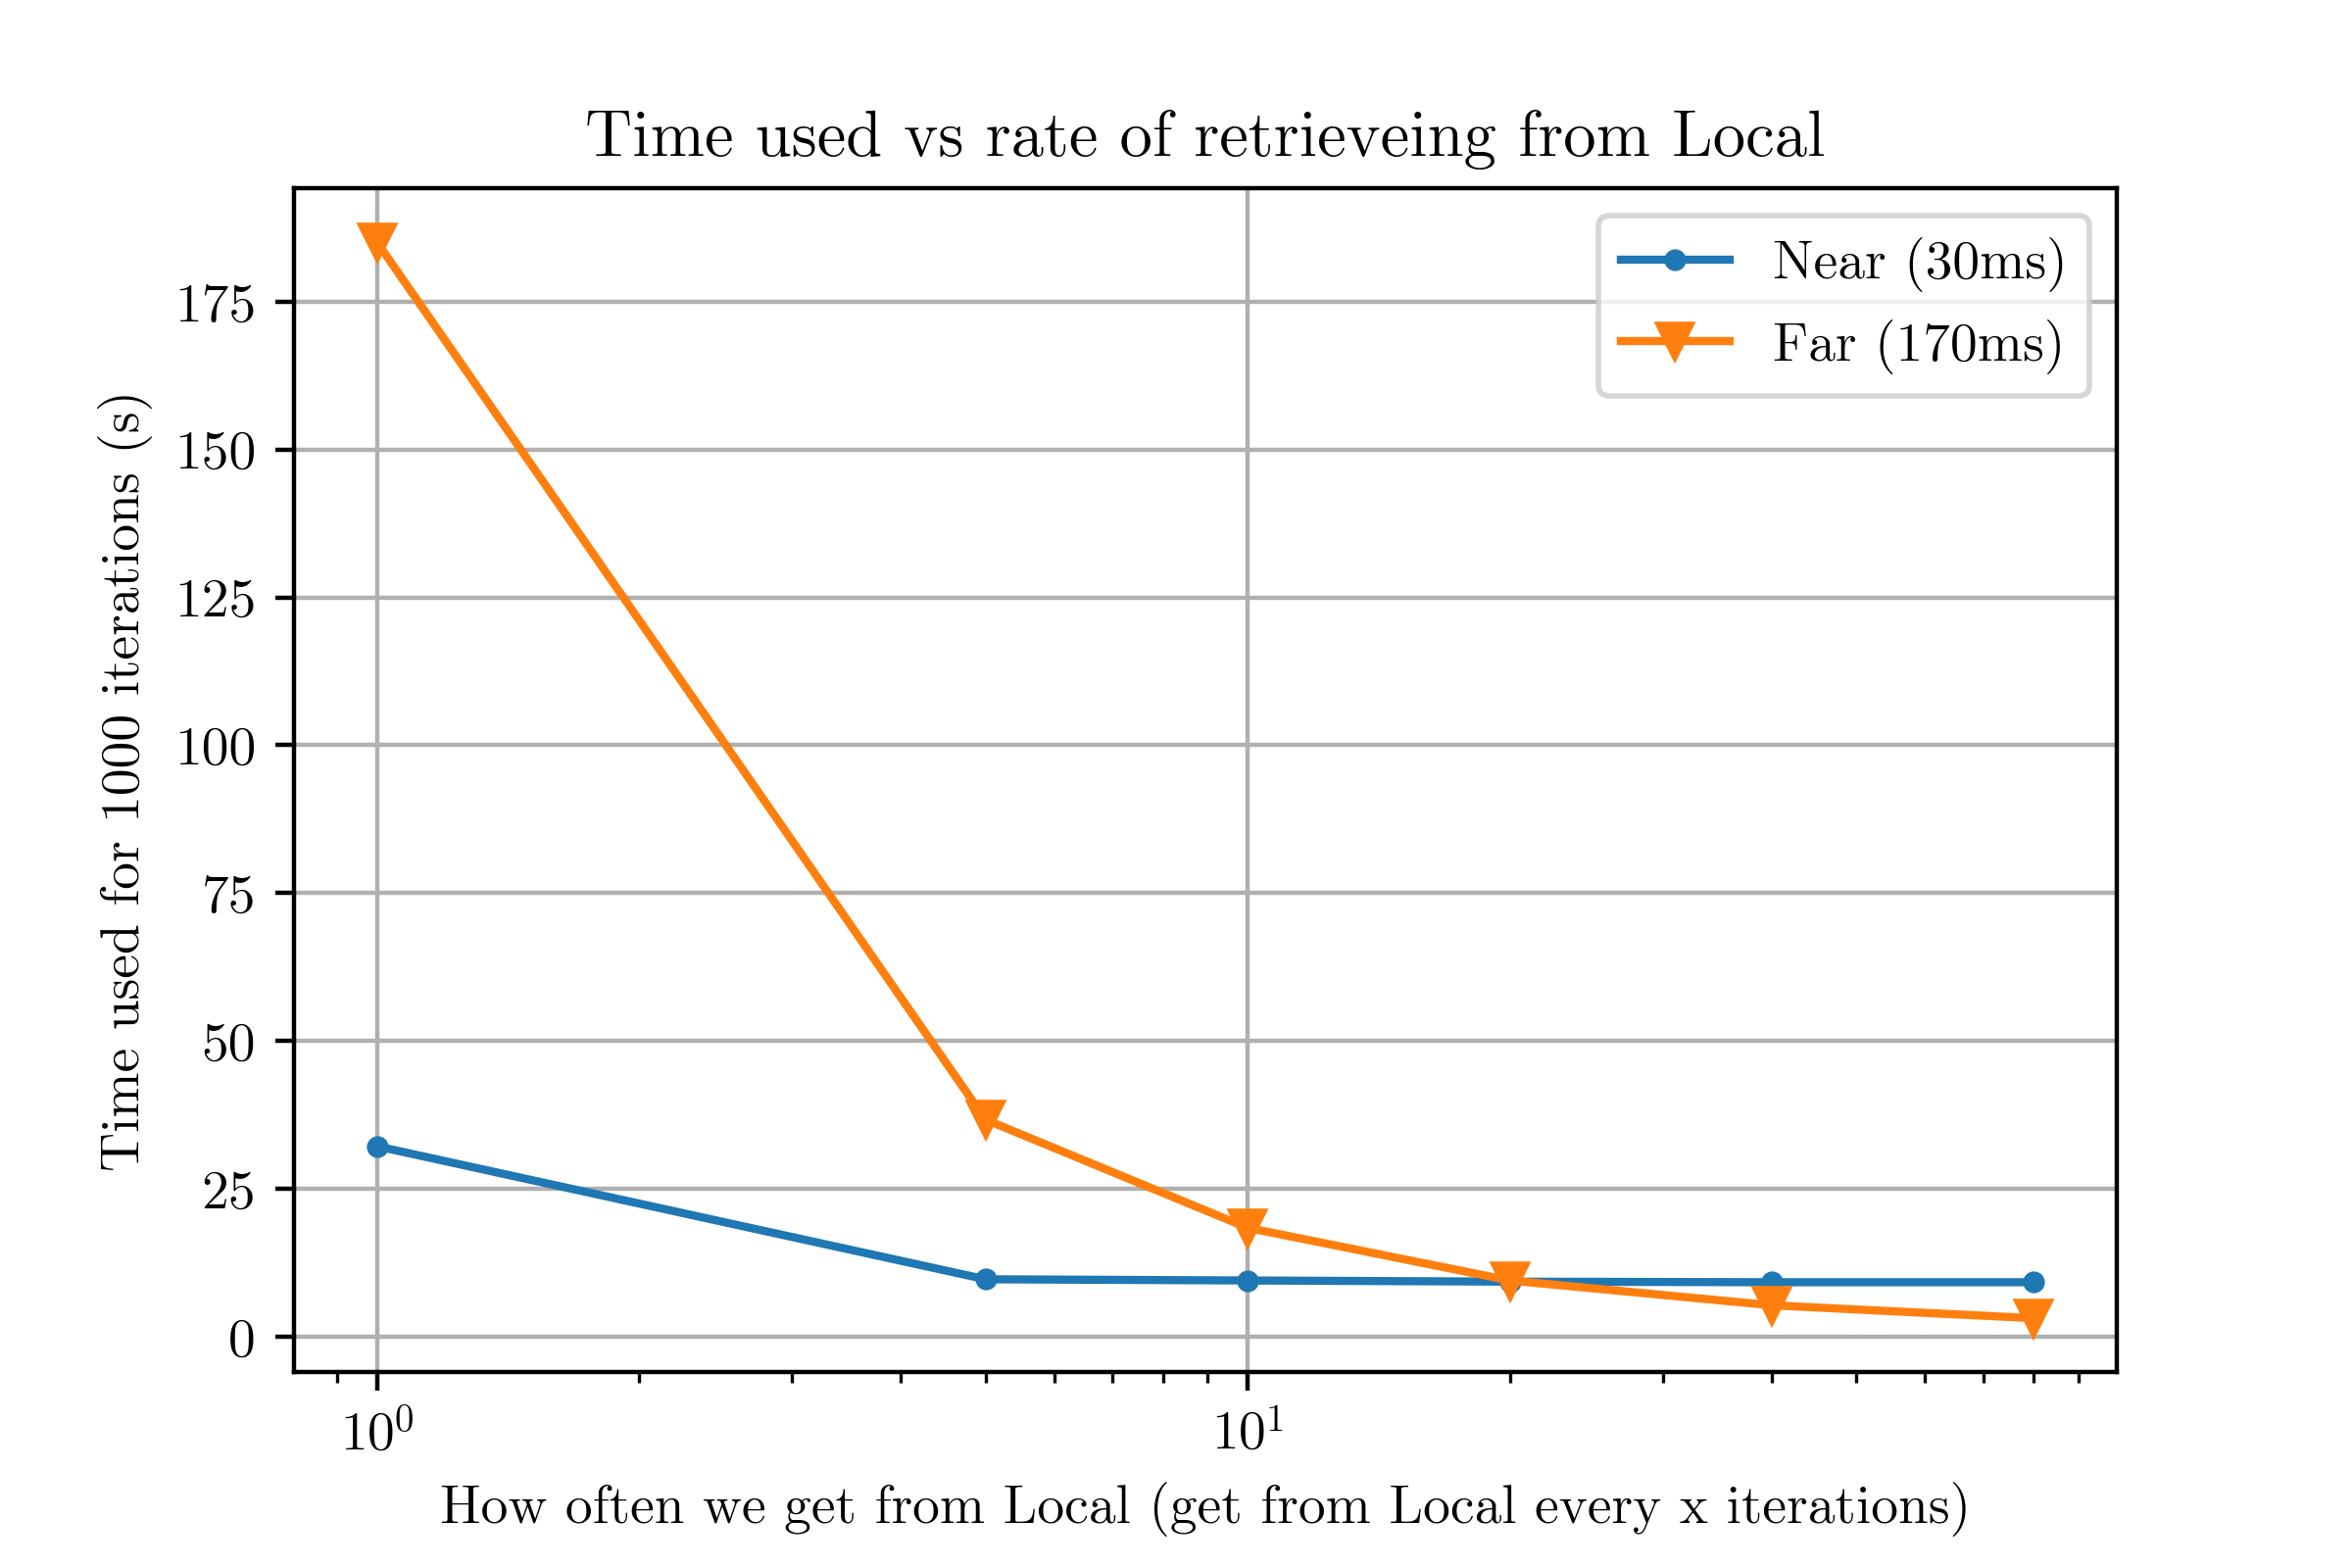
\includegraphics[scale=1]{chapters/evaluation/figures/times.png}
    \caption{Graph showing how interaction hurts. If x=10 then we get from Local every 10 iterations.}
    \label{fig:time_graph_near_far}
\end{figure}

Figure \ref{fig:time_graph_near_far} shows how latency affects the time used when you have to constantly get data from the Local device. We have tested with various frequencies of interaction. The graph essentially shows how much time is used on Near or Far node with regards to how often it has to get data from the Local node. 
\begin{figure}[t]
    \centering
    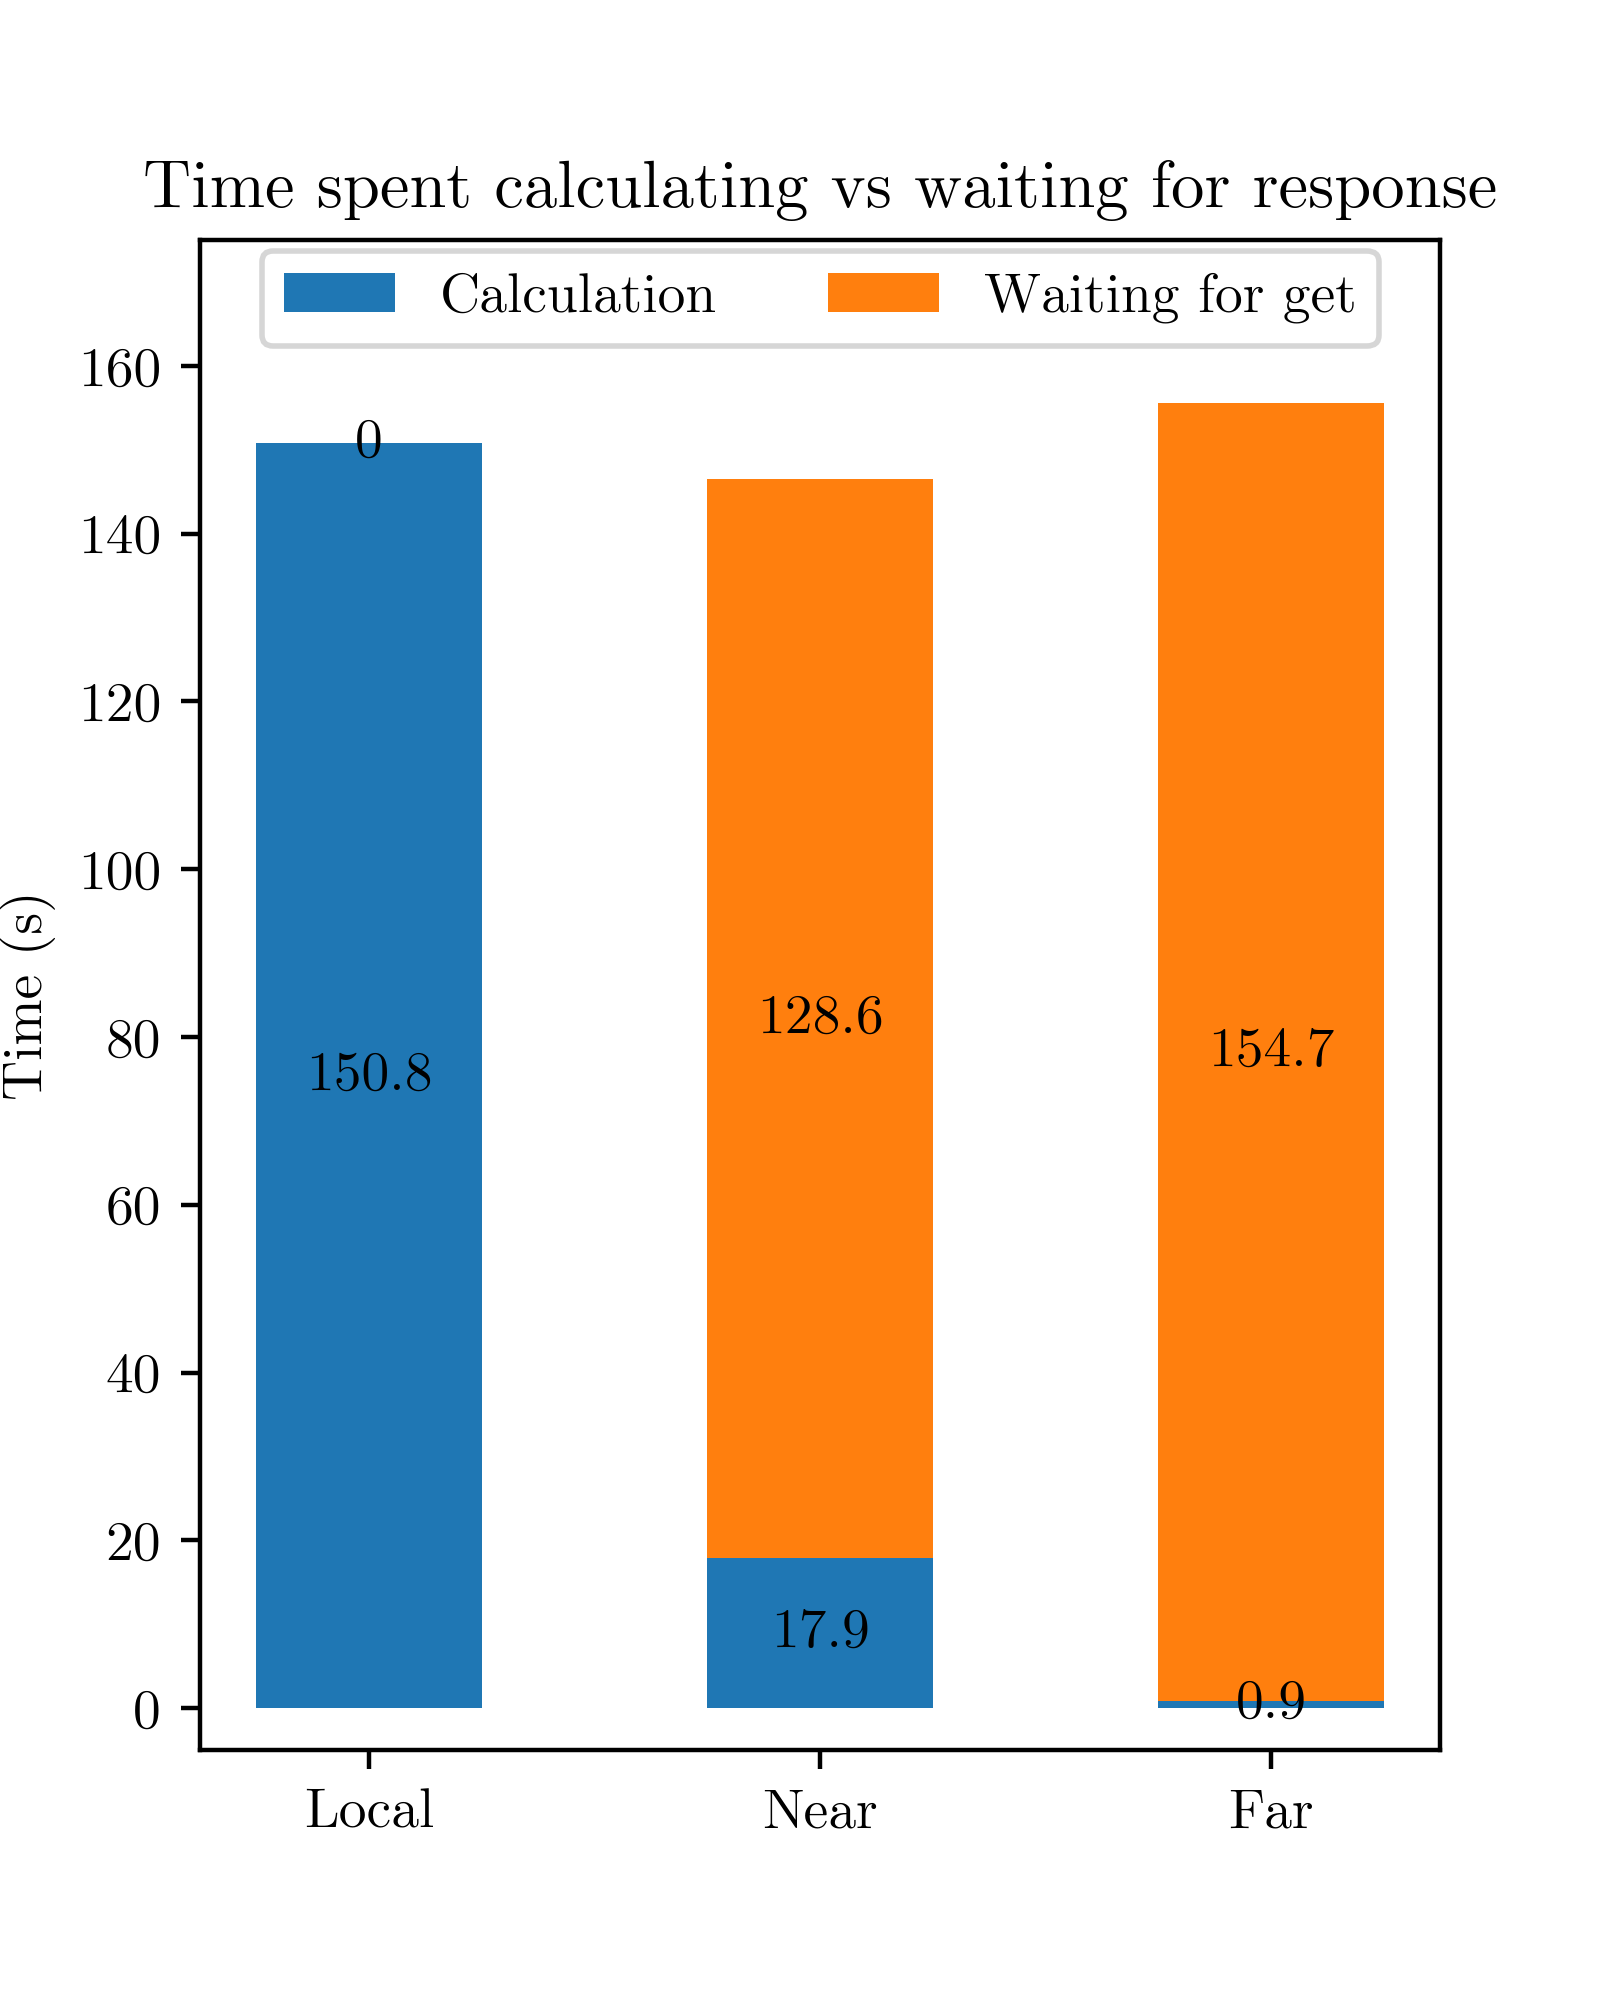
\includegraphics[scale=1]{chapters/evaluation/figures/bar_local_near_far_compare.png}
    \caption{Illustration of how much time is spent on waiting for data due to latency when using MEC Server.}
    \label{fig:bar_local_near_far}
\end{figure}

Figure \ref{fig:bar_local_near_far} shows how latency affect the the total time used when we have to constantly get data from the local device. It uses the same configuration as shown in table \ref{tab:MEC_partial_offloading_latency_balance}.


\begin{table}[h!]
    \centering
    \begin{tabular}[c]{|c|c|c|c|c|}
        \hline
        Node type & Limitation & Iterations & RTT to Local (ms)& Time used (s)\\
        \hline
        \hline
        Local & 30 & 850 & 0 & 28.0  \\
        \hline
        Near & 100 & 850 & 30 & 27.6 \\
        \hline
        Far & 300 & 8300 & 170 & 27.5 \\
        \hline
    \end{tabular}
    \caption{Partial offloading with a lot of communication between Local and Near, and little communication with Far.}
    \label{tab:MEC_partial_offloading_little}
\end{table}

Table \ref{tab:MEC_partial_offloading_little} shows the result of having high frequency of interaction between Local and Near, while having low frequency of interaction with Far.



\subsection{Discussion of results} \label{subsection:MEC_comparison}%Discussion of mec?
By comparing table \ref{tab:MEC_full_offloading_latency_balance} and \ref{tab:MEC_partial_offloading_latency_balance} we can see that we get faster results by using Partial offloading. Because the nodes work in parallel, the node who used the longest time shows how much time were used from start to end. Therefore, Partial offloading is the best solution for having fastest result when there is a lot of interaction.


Full offloading might for some devices be a requirement. The two most likely causes for this is if the Local device have very limited computational power, or need to save battery. Computation offloading is a great strategy to save energy, as sending data is usually not as expensive as computation. However, if we compare table \ref{tab:MEC_full_offloading_latency_balance} and \ref{tab:MEC_partial_offloading_latency_balance}, we can clearly see that using the local device will give results faster.

Table \ref{tab:MEC_partial_offloading_little} shows that using a strong Far node is beneficial as long as the interaction between Local or Near and Far is low. Additionally, figure \ref{fig:bar_local_near_far} shows that if the Near and Far node constantly have to get data from Local, the time to complete the whole task will be much slower. If you don't need to get info that often, then the Far server will yield better results as it has more computational power. In other words, the more interaction the better it is to use Local or Near node more. When there is little interaction then it is best to use the Far node more.

%nevn offloading. Vis stolpediagramm hvor en chunk av tiden er offloading. Vis også med N*latency?
%Bar chart med som viser hvor stor andel av de forskjellige utregningene som består av calulation og latency






\subsection{Characteristics}
\subsubsection{Control}
As discussed in section \ref{section:MEC_architecture}, the network architecture of MEC is up to the programmers. They can use NFV and SDN to control how each mobile device will be able to use the architecture. They can in other words use SDN and NFV to tailor the network to the context. Since VMs can be uploaded to surrounding MEC Servers, ensuring good \textit{relocation transparency} should be trivial. Due to SDN and NFV they could quickly redirect packets to new MEC Server when needed. The level of \textit{migration transparency} is therefore also left to developers.

\subsubsection{Offloading}
Since they use the cellular network to offload work, this architecture is well suited for IoT devices that can afford the latency. The cellular network is ubiquitous in modern society, and therefore it is optimal for IoT devices that move a lot, e.g. self-driving cars. When offloading they have to upload something, e.g. a VM, to the MEC Server. Alternatively they can make the MEC Server download from elsewhere. Since MEC uses VMs on the servers when offloading, the level of \textit{access transparency} is very good. The VMs ensure that the APIs for all the nodes are the same. Since cellular networks cover such a large area, \textit{location transparency} is trivial as the device can move quite a lot of distance before any migration is needed. If a node were to fail, it is up to the developers to ensure that other resources are available to recover from the failure. In other words, the level of \textit{failure transparency} is up to the programmers.

\subsubsection{Deployment}
MEC is easily horizontally scalable, as more MEC Servers can easily be added to cell towers. The only limit is how much power there is available and how much space there is available. If only a few servers is needed, then the cost is not too high either. It is also easily scalable in the sense that you can add more VMs to the MEC Server to help with offloading if needed. Another benefit of using VMs is that \textit{concurrency transparency} is easy to ensure as long as the MEC Server does not run out of resources. This is because they are in sperate VMs and should not affect each other.



%offloading
%    compute 
%    storage
%distribution
%    scaling
%Control


%tabell? subsections? idk

%TODO
% Gjøre målinger med overføring av filer først. Finn data på bandwidth og pluss det på tiden.
% Gjøre målinger hvor det kreves mer samhandling mellom nodene. Vi må se latency!


%\cite{mach_mobile_2017} for hvor mye som skal offloades.!!!!
% test med 100% offload, 50% offload osv
%\begin{itemize}
 %   \item Easily scalable as we have the common interface. This makes it easy to add more vms to run more apps. So, its horizontally scalable?
%\end{itemize}





% -------------------------------------------------------------------------------------------





\section{Cloudlets}
For Cloudlets we will also test with Full and Partial offloading like in section \ref{section:MEC_evaluation}. The same metrics for limitations for each type of node is also used. In total we want to do 10000 iterations spread over all the nodes.

\subsection{Full execution}
\begin{table}[h!]
    \centering
    \begin{tabular}[c]{|c|c|c|c|c|}
        \hline
        Node type & Limitation & Iterations & RTT to Local (ms)& Time used (s)\\
        \hline
        \hline
        Local           & 30 & 0 & 0 & 0  \\
        \hline
        Cloudlet(Near)  & 100 & 2800 & 3 & 30.2 \\
        \hline
        Far             & 300 & 7200 & 170 & 1285.0 \\
        \hline
    \end{tabular}
    \caption{Full offloading with communication.}
    \label{tab:Cloudlet_full_offloading_latency}
\end{table}
Table \ref{tab:Cloudlet_full_offloading_latency} shows the result of Full offloading to a nearby Cloudlet. We have used the same configuration as in table \ref{tab:MEC_full_offloading_balanced} to show how latency affects the result. 

\begin{table}[h!]
    \centering
    \begin{tabular}[c]{|c|c|c|c|c|}
        \hline
        Node type & Limitation & Iterations & RTT to Local (ms)& Time used (s)\\
        \hline
        \hline
        Local           & 30 & 0 & 0 & 0  \\
        \hline
        Cloudlet(Near)  & 100 & 9500 & 3 & 98.8 \\
        \hline
        Far             & 300 & 500 & 170 & 94.6 \\
        \hline
    \end{tabular}
    \caption{Full offloading with communication with more balance.}
    \label{tab:Cloudlet_full_offloading_latency_balanced}
\end{table}
Table \ref{tab:Cloudlet_full_offloading_latency_balanced} shows the result of a more balanced configuration with Full offloading in the sense that they used about the same time.




\subsection{Partial offloading}
\begin{table}[h!]
    \centering
    \begin{tabular}[c]{|c|c|c|c|c|}
        \hline
        Node type & Limitation & Iterations & RTT to Local (ms)& Time used (s)\\
        \hline
        \hline
        Local           & 30 & 850 & 0 & 28.1  \\
        \hline
        Cloudlet(Near)  & 100 & 2700 & 3 & 27.8 \\
        \hline
        Far             & 300 & 6450 & 170 & 1188.4 \\
        \hline
    \end{tabular}
    \caption{Partial offloading with communication.}
    \label{tab:Cloudlet_partial_offloading_latency}
\end{table}
Table \ref{tab:Cloudlet_partial_offloading_latency} shows the result of Partial offloading to a nearby Cloudlet. We have used the same configuration as in table \ref{tab:MEC_partial_offloading_balanced} to show how latency affects the result. 





\begin{table}[h!]
    \centering
    \begin{tabular}[c]{|c|c|c|c|c|}
        \hline
        Node type & Limitation & Iterations & RTT to Local (ms)& Time used (s)\\
        \hline
        \hline
        Local           & 30 & 2400 & 0 & 79.2  \\
        \hline
        Cloudlet(Near)  & 100 & 7150 & 3 & 73.3 \\
        \hline
        Far             & 300 & 450 & 170 & 75.2 \\
        \hline
    \end{tabular}
    \caption{Partial offloading with communication with more balance.}
    \label{tab:Cloudlet_partial_offloading_latency_balanced}
\end{table}
Table \ref{tab:Cloudlet_partial_offloading_latency_balanced} shows the result of a more balanced configuration with Partial offloading in the sense that they used about the same time.







\subsection{Decreasing interaction}
\begin{figure}[t]
    \centering
    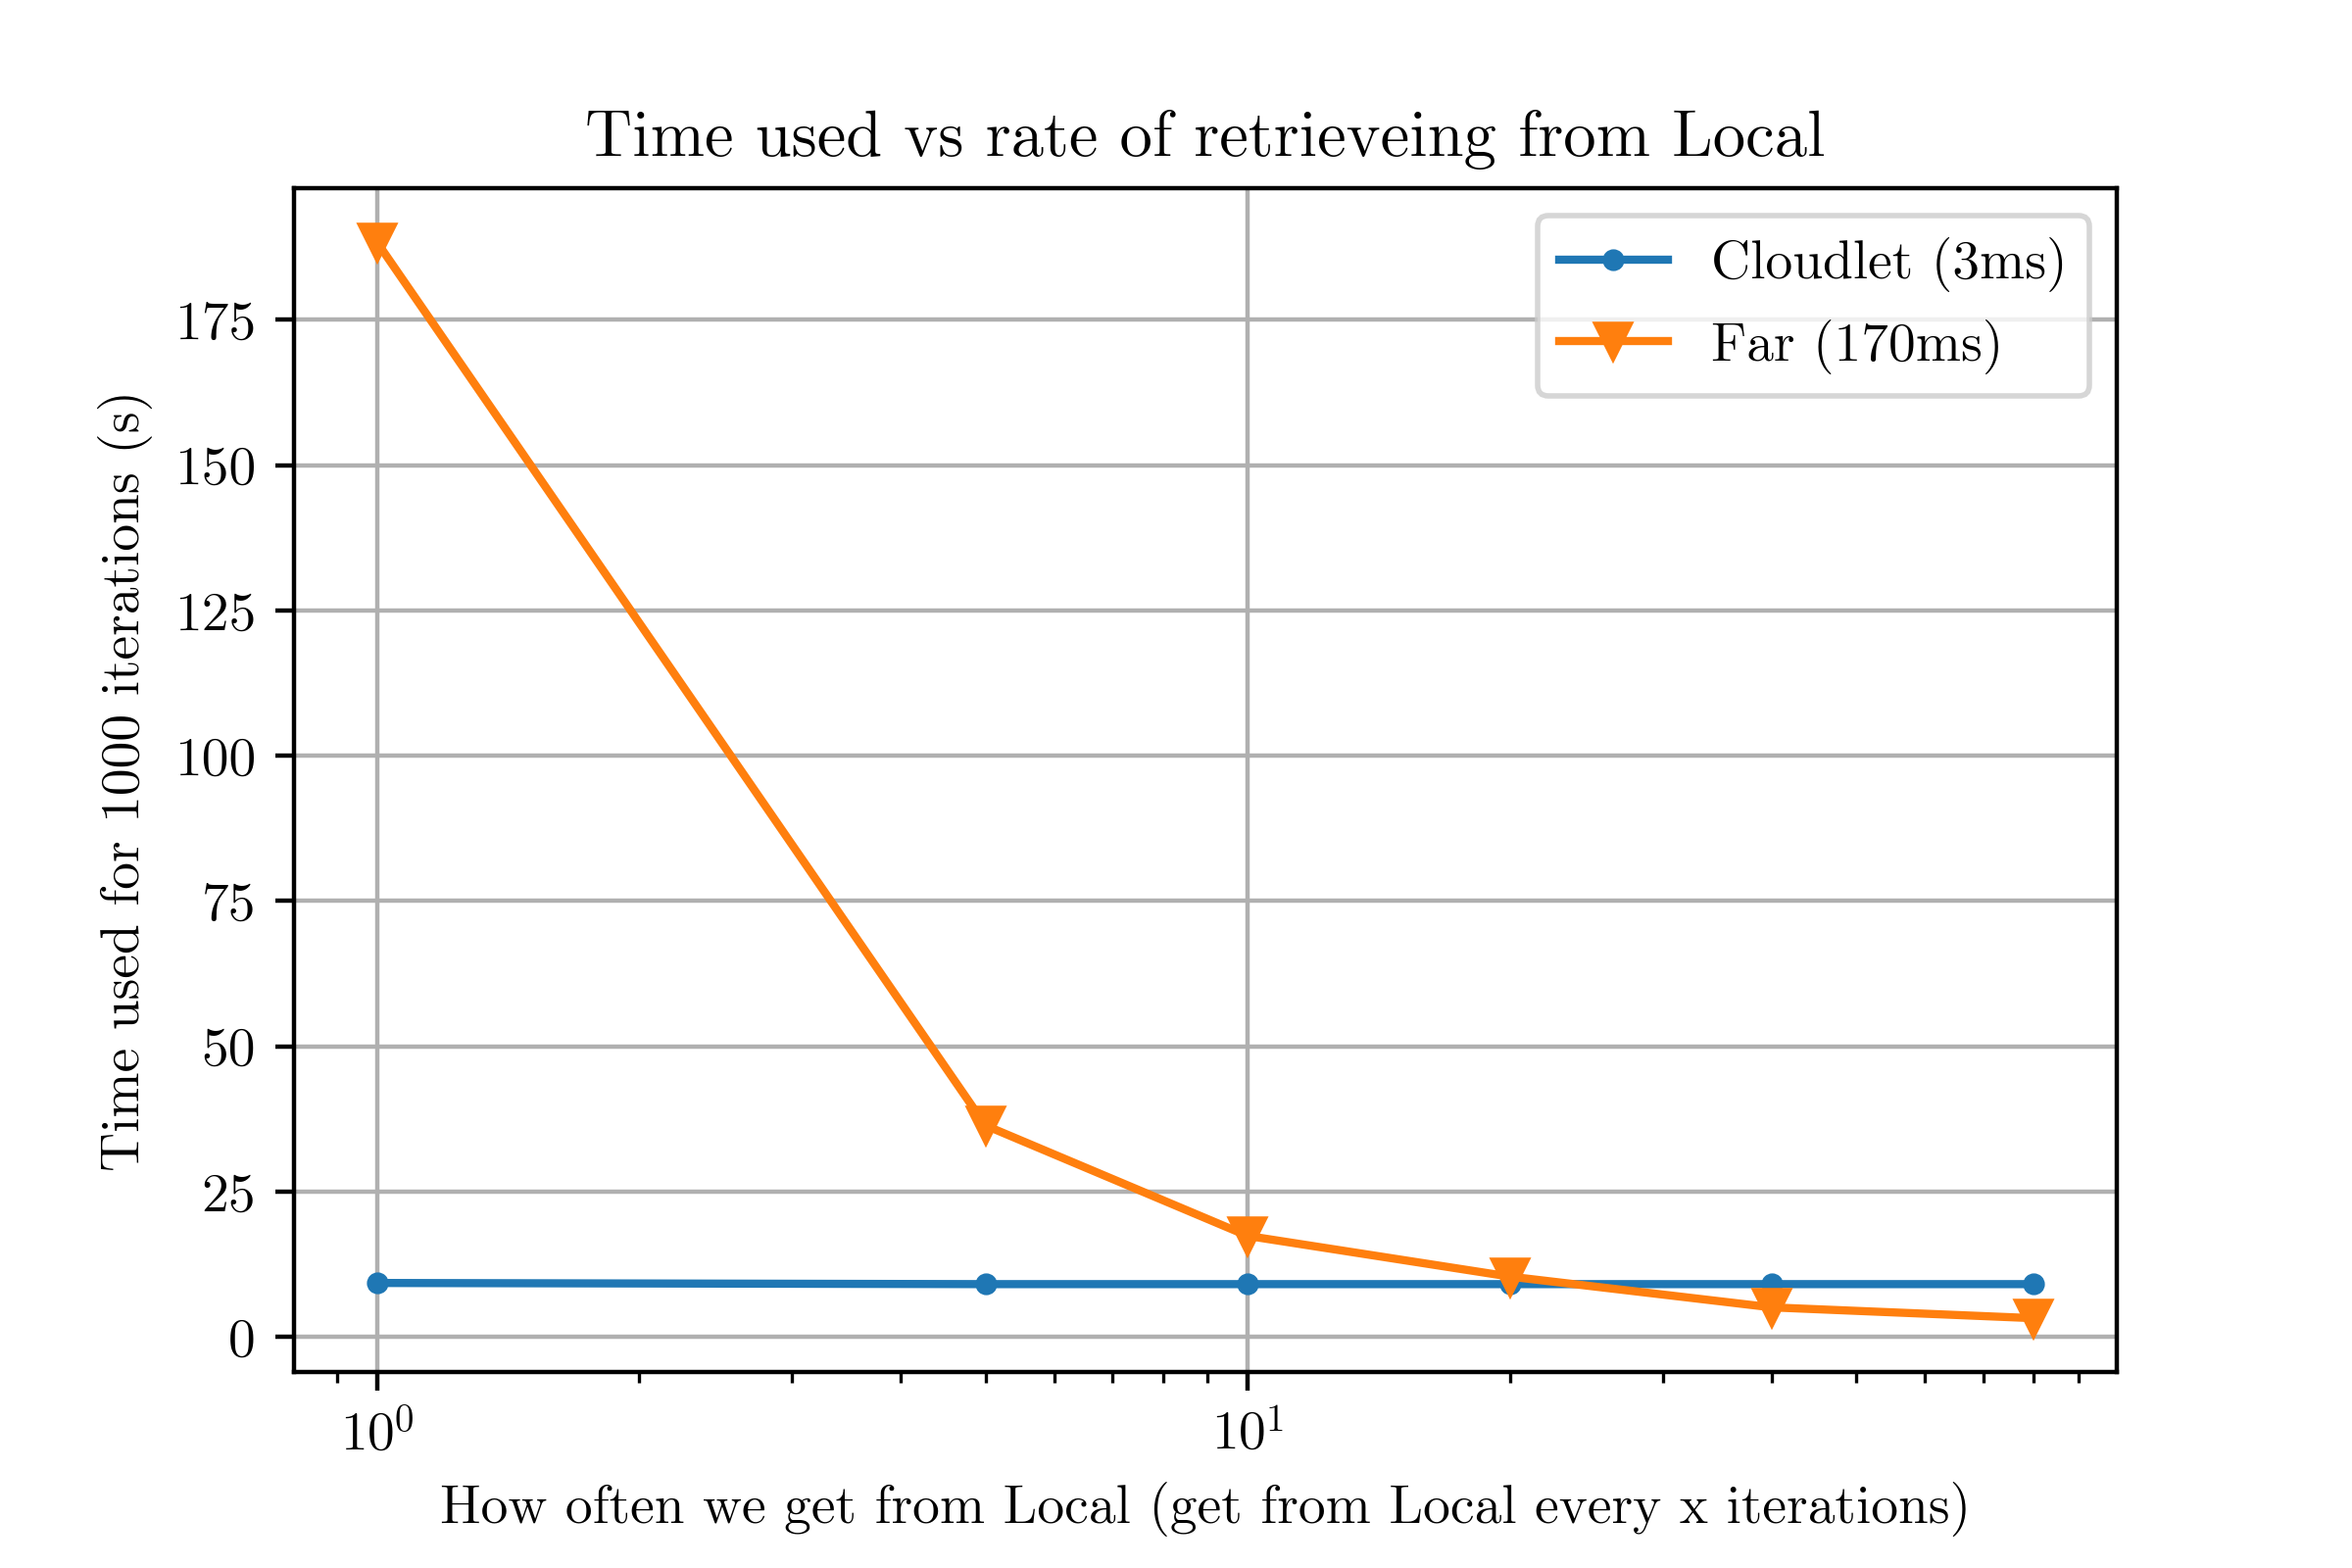
\includegraphics[scale=1]{chapters/evaluation/figures/Cloudlet_latency.png}
    \caption{Graph showing how interaction hurts. If x=10 then we get from Local every 10 iterations.}
    \label{fig:Cloudlet_latency_near_far_comparison}
\end{figure}
Figure \ref{fig:Cloudlet_latency_near_far_comparison} shows how the frequency of interaction between nodes will affect the time used, like shown for MEC in \ref{fig:time_graph_near_far}. 


\begin{figure}[t]
    \centering
    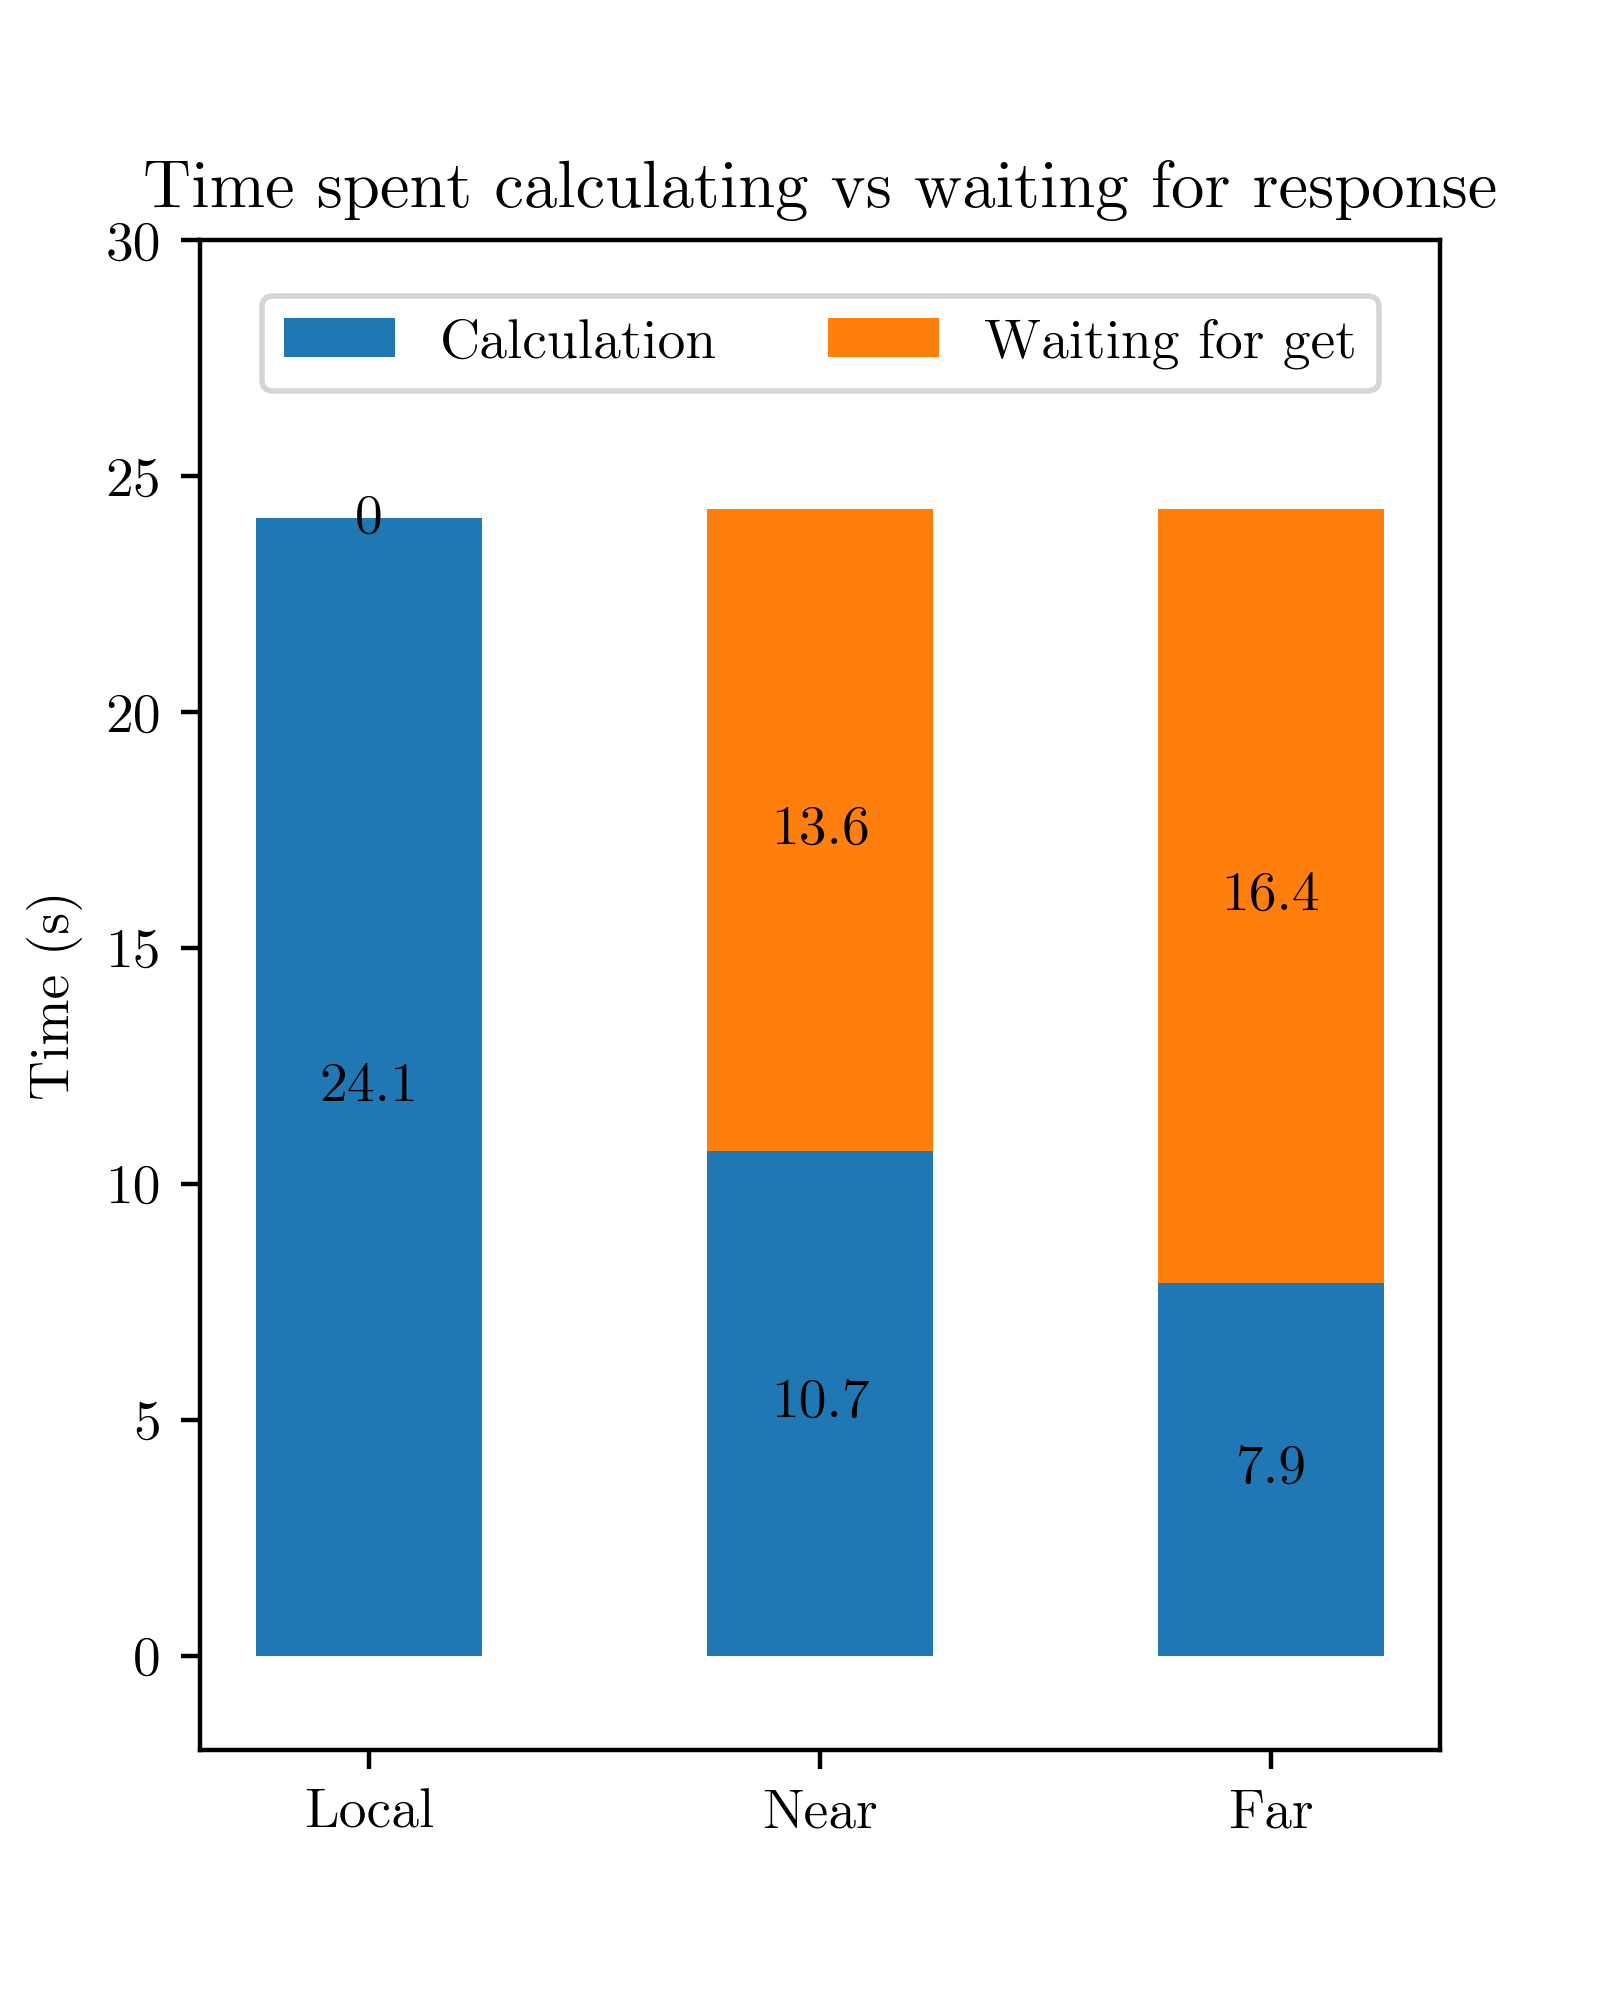
\includegraphics[scale=1]{chapters/evaluation/figures/bar_local_near_far_compare_low_interaction.png}
    \caption{Illustration of how much time is spent on waiting for data due to latency when using Cloudlets.}
    \label{fig:Cloudlet_latency_bar}
\end{figure}
Figure \ref{fig:Cloudlet_latency_bar} shows how much time used on waiting for data from Local, compared to how much time is used on calculating. The configuration used here is the same as shown in table \ref{tab:Cloudlet_partial_offloading_latency_balanced}.


\begin{table}[h!]
    \centering
    \begin{tabular}[c]{|c|c|c|c|c|}
        \hline
        Node type & Limitation & Iterations & RTT to Local (ms)& Time used (s)\\
        \hline
        \hline
        Local           & 30 & 750 & 0 & 24.1 \\
        \hline
        Cloudlet(Near)  & 100 & 2250 & 3 & 24.4 \\
        \hline
        Far             & 300 & 7000 & 170 & 24.3 \\
        \hline
    \end{tabular}
    \caption{Partial offloading with a lot of communication between Local and Near, and little communication with Far.}
    \label{tab:Cloudlet_partial_offloading_little_far}
\end{table}
Table \ref{tab:Cloudlet_partial_offloading_little_far} shows the result of offloading with high frequency to the Near node, while letting the Far node have bigger workloads, and therefore frequent interaction. 


\subsection{Discussion of results}
By comparing table \ref{tab:Cloudlet_full_offloading_latency_balanced} and \ref{tab:Cloudlet_partial_offloading_latency_balanced} we can see that we benefit from also using the Local device. However, if the device that is using the Cloudlets require Full offloading, then we still have significant speedup by offloading to the Cloudlet and the Far node compared to Local execution. Table \ref{tab:Cloudlet_partial_offloading_little_far} shows that using Far node as long as interaction is low, is also very beneficial.

Figure \ref{fig:Cloudlet_latency_near_far_comparison} shows that we can get better results by using Far in the situation where interaction between nodes is low. In other words, Cloudlets can benefit from using Far, but only when there is little communication needed. For fast response times we need to use the Cloudlet to do the computation. 

Figure \ref{fig:Cloudlet_latency_bar} shows that having minimal latency to a Near node is very beneficial. Even though almost half of the time is spent waiting, we have offloaded a significant amount of work. Table \ref{tab:Cloudlet_partial_offloading_little_far} 



\subsection{Characteristics}
\subsubsection{Control}
Controlling Cloudlets is done by the owner of each Cloudlet. Since Cloudlets are to be placed on locations, e.g. a coffee shop, then the owner of that location is able to configure the Cloudlet. The location owner can then limit usage and limit what kinds of applications are used on the Cloudlet. Handling failure and having good \textit{failure transparency} is mostly up to the programmer in Cloudlets. Should the Cloudlet fail, then a different near Cloudlet should take over, or in the worst case let the Local device handle it. 
\subsubsection{Offloading}
Cloudlets use \textit{dynamic VM synthesis} \cite{satyanarayanan_case_2009} to offload work. Essentially it means that we have to give the Cloudlet a VM to run the application. This makes \textit{access transparency} for Cloudlets quite good in theory. However, it gives an overhead which they reported to be quite high. This has likely been improved since 2009 as technology has improved. Bandwitdth, storage and computational power have significantly improved, which mitigates many of the issues they raised.
\subsubsection{Deployment}
Distribution is expensive for Cloudlets. Satyanarayanan et al\cite{satyanarayanan_case_2009} purposes different payment models, but each owner of a location has to decide if it is worth the investment. Since they are supposed to be ubiquitous, the total cost of having these readily available everywhere in society will be significant. If the Cloudlets are ubuiquitus, then the level of \textit{location and relocation transparency} is quite high. In their paper, they purpose a way of seamlessly migrating to other Cloudlets when needed. If this is accomplished, then the users of the local devices will not notice any drop in performance. Due to the ubiquitous nature of Cloudlets, having \textit{concurrency transparency} should not be a problem. Overloading all of the nearby Cloudlets will be a rare occurrence due to their ubiquitous nature.







% -------------------------------------------------------------------------------------------







\section{Google Anthos}
\subsection{Characteristics}
\subsubsection{Control}
Controlling the Anthos architecture is relatively easy as GCP will take care of all the difficult parts. You can control all the nodes in the Anthos control panel. This means that the one who owns the GCP account has full control over the nodes. The level of \textit{access  transparency} is quit high, as Anthos will take care of all the low-level problems. It is up to the programmer to decide how containers running on the platform will communicate. It also up to the programmer if they want users to be able to relocate objects. In other words \textit{migration transparency} is also up to the programmers.

\subsubsection{Offloading}
Since Anthos uses containers, offloading can be quite easy. However, it is up to the programmers to decide how offloading will work. Essentially, the Local device only needs to somehow contact the on-premises machines, for example through WiFi and LAN connections. The level of \textit{location transparency} is up to the programmers. It is dependent on how the containers are set up. Kubernetes is easily set up to manage \textit{replication and concurrency transparency}, as it lets you configure where the containers should reside, and how many of them should be there, as well as many other parameters.

\subsubsection{Deployment}
Deploying is relatively easy. As discussed earlier, you only need to install Anthos software on on-premises hardware and then configure Kubernetes to use it. Ensuring \textit{failure transparency} can be hard, but Kubernetes is configureable to handle failures. Essentially, it is up to the programmer to decide what happens if there is one.






% -------------------------------------------------------------------------------------------







\section{Amazon Cloudfront}
\subsection{Characteristics}
\subsubsection{Control}
Controlling Cloudfront is done in the Cloudfront control panel in the AWS console. Cloudfront lets you set up a wide array of features for your architecture. They provide DNS, NFV, Lambda@edge, Security, Sertificates, etc. All of this is controlled by the programmers in the AWS console.  


\subsubsection{Offloading}
AWS lets you set up servers, container software or Lambda@edge on Cloudfront. This lets gives a lot of freedom to the programmers on how they will set up the architecture. A downside of using AWS Lambda is that there is something called warm up time. It is pretty small, but can be notices in extreme latency-aware contexts. The warm up time depends on the programming language used, but it comes in addition to the latency towards the edge location. When it comes to \textit{concurrency, location and replication transparency}, it is up to the programmer, but are very easily adjustable. For example, for AWS Lambda, a single parameter can be change to let it scale more. AWS will handle scaling, the programmer just have to set the limit. When using server however, you have to add more servers to scale, so it is therefore more up to the programmers. The level of \textit{access transparency} is high, due to containerization and AWS Lambda. However, if servers are used, then the programmer have control of the access transparency level. \textit{Relocation and migration transparency} can be ensured by Cloudfront, unless you use the servers. Then it is up to the programmer to control it. 


\subsubsection{Deployment}
When setting up Cloudfront you do it trough the AWS control panel. You are restricted to use the edge servers that AWS provide. These servers are deployed all over the world. However, in some places there might be a long distance to the nearest server. Ensuring \textit{failure transparency} is handled by Cloudfront in this architecture. The programmer can focus more on what the program should do rather than focusing on what happens if it were to fail. 




% -------------------------------------------------------------------------------------------





\section{Akamai}
\subsection{Characteristics}
\subsubsection{Control}
Akamai features are controlled through Akamai's console. The level of \textit{access and migration transparency} is up to the programmer in this architecture.

\subsubsection{Offloading}
Akamai does offer ways of offloading, but they focus more on bringing content to the edge rather than just computation. Caching is the main purpose of Akamai edge servers, and using their edge servers for this ensures \textit{location, relocation, replication and concurrency transparency}. The level of \textit{replication transparency} is also somewhat up to the programmer, as the choose the locations of where they should cache the content.

\subsubsection{Deployment}
Setting up the edge servers are easily done through Akamai's console. You set up the edge server where you want it, and then push your content to that server. Akamai will take care of failures and will route requests to the original server if needed. This ensures \textit{failure transparency}. However, if the orginial server is very distant, then the client will most likely notice a drop in performance or response time.


% -------------------------------------------------------------------------------------------




\section{Discussion of findings}

\subsection{Comparing Cloudlets and MEC}
From the results we can see that if enough funding is available, then Cloudlets gives the best result. We can see that having low latency between Local and Near like the Cloudlet, is preferable for better results. However, one could argue that installation of MEC Servers are significantly easier and cheaper as you only install them at base stations that cover a wide area. When it comes to migration, it is significantly easier for MEC due to how much area is covered with cellular. If the mobile device were to move in the Cloudlet architecture then Cloudlets in the new location should already be ready to offload. This is hard, as with the frequency of Cloudlets it can be difficult to decide which Cloudlet to migrate to before it is too late. Since MEC cover such a large area, it should not be a problem to see when it is needed to migrate to other base stations. However, migration in MEC will likely take a longer time, as Cloudlets often will be on the same LAN and can therefore transfer faster and more reliably.

\subsection{Discussion of architectures}
Anthos is able to mimic the Cloudlet architecture by letting you set up on-premises servers. However, the Anthos nodes are confined to the owners environment, which is unlike the vision for Cloudlets. 

Cloudfront is a good choice as it is backed by a massive company, which has infrastructure in a lot of locations, and will likely expand in the future. It comes with the negative side effect of being confined to their locations, which in many cases might have too much latency.

Akamai is leading when it comes to content caching as they have the most infrastructure available. However, it is best used as a standard CDN, in the sense that you should offload web pages or other high volume data to their servers. Doing this will significantly improve the response time due to the lower latency, and will most likely give a smoother experience as there is less use of the Wide-area network.

A common thing for all architectures is that a lot of the control is up to the programmers. This allows for high customization of the application, as it is not limited to many constraints. Additionally, all the architectures allow for cooperation between Near nodes and Far nodes. 


\subsection{Offloading}
We can see from table \ref{tab:MEC_partial_offloading_little} and \ref{tab:Cloudlet_partial_offloading_little_far} that we do get a speed-up by using the Near-Far model, on the condition that the Far node does not do much latency-aware work. 

Every architecture that requires transferring of a VM or similar to the offloading node, will have an overhead. This overhead is mainly dependent on the size of the load that need to be transferred, the bandwidth between the Local and Near node, and the time it takes to start the VM or container. Context is required to know when to start offloading these VMs to the other nodes. If context is well known to the nodes, then they can start pre-loading to avoid having to wait for this overhead.







\section{The Near-Far Computing Model}
The Near-Far Computing Model is worth it in many cases. However, it is best utilized when you can have a Near node doing latency critical work, and having a Far node doing the latency non-critical work. For example, if the Local device is a smart device that need quick response on their data, it can offload to the Near node. When the Near node is done calculating, it can use the Far server to analyze the result as well as logging it. For storage, Near-Far is great for caching. Having caches that is closer to the client will result in way quicker results.

The common thing for all the discussed architectures is that they use a mix of both edge nodes and server nodes. They try as best as possible to use the edge nodes, but the distant strong data centers can aid when needed. 

If the Near node were to fail, then the Far node can take over. However, due to latency the Far node will give the client a worse experience if response time is critical. 

\subsection{Distribution Transparency}
In the following subsections we will discuss distribution transparency in Near-Far computing.

\subsubsection{Access Transparency}
When using the Near-Far model, one should use containerization or VMs to provide common API or middleware for all the nodes in the system. This ensures that developers does not have to deal with very low-level programming, and focus more on providing features and solutions.

\subsubsection{Location Transparency}
Location transparency is up to the programmer, but in most cases one should try to hide where objects are located. Due to the Near node having low latency, there should not be a problem to ensure that the location is hidden.

\subsubsection{Relocation Transparency}
Relocation transparency can be hard if the area where you are connected to the Near device is not big. For example, if you have to connect to a new node each time you enter a new room, ensuring relocation transparency can be hard. However, with good algorithms and enough knowledge about the context, it is possible. 

\subsubsection{Migration Transparency}
Migration transparency should not be difficult to implement. It is up to the programmer to decide how much level of transparency they want. 

\subsubsection{Replication Transparency}
Replication transparency is mostly up to the programmer. With enough Nodes available, the programmer can add or remove nodes as they see fit. It is up to the context if this will be noticed by the client. 

\subsubsection{Concurrency Transparency}
Concurrency transparency is also up to the programmer. In most cases however, it is best to avoid showing that multiple users are using the same resources. For example, one should not notice that several others are watching the same content as you are. 

\subsubsection{Failure Transparency}
If enough nodes are available, then recovering from a failure should have minimal impact on the user. However, if the application in question is latency-aware and is forced to use Far or Local resources to do these time critical operations, then the client will suffer. However, one should quickly be able to recover to the previous state.

\subsection{Definition}
The Near-Far Computing is a superset, or a spectrum that covers all models or architecutres that focuses on mitigating latency issues by using Near nodes and Far nodes. 



\section{Summary}
In this chapter we have tested MEC and Cloudlets with the program described in implementation. We have also discussed characteristics of all the architectures. We have discussed how these characteristics relate to the Near-Far Computing Model. Finally we have provided a definition for the Near-Far Computing Model



\section{TODO}

Sometimes the result of the far is not relevant for the near. We can also let the near compute while the far stores data.

Near-Far computing is applicable where there is not much need for interaction between the Far node and the Local or Near node.

